\section{Development Models}
There are many development models in the field that are inspired by nature. Though the concept of biological development does not change much, it is very much still a topic under discussion and there are still uncharted territories. It is therefore not surprising that these models differ not only in implementation, but also the biological ideas behind it. In this chapter, we will take a look at two models. We'll see how they work, and discuss their differences. These models are important for this thesis because they are believed to represent the greatest difference in development models to date. The reason behind this is to make sure the framework will cover as much ground as possible. Because it is intended to be generic, it would be sad if a model did not fit in. This chapter will only go into the concepts that these models are based. More detailed and technical walkthrough will be saved for the next chapter, where they are re-implemented.

\subsection{ArtDev3D}
\label{sec:Models:ArtDev3D}
In 2006, Johan H{\o}ye handed in his master's thesis\cite{hoye2006} based on his own model of biological development. Its aim was to draw inspiration from biology but simplify concepts to avoid dwelling too deep into the underlying and less understood concepts. His model relies on DNA with a small control program in the cells.

\subsubsection{Concepts}
To understand this model, we will have to touch a few topics in biology. Like with humans, everything starts out with a single cell, the zygote. The zygote divides and the organism has grown to consist of two cells. These cells divide again to become four cells. This process repeats itself in a controlled fashion with the help of the DNA, the recipe of life. It tells which proteins to synthesize, how and when. The proteins, in turn, carry out all the actual work inside the cell. In his model, only four such tasks were defined at the time, though more could have been added:

\begin{itemize}
	\itemsep=0pt
	\item Change the type of the cell
	\item Regulate chemical levels
	\item ``Request'' cell division in several directions
	\item Synthesize/transcribe more proteins
\end{itemize}

I use ``request'' here because of the way this model works. The proteins queue a request for the cell to perform division in some directions. These requests are accumulated and if the stimuli levels are above a given threshold, it will be actualized. The accumulation works like a voting system, once there are enough votes for a particular direction, cell division will occur in that direction. The only difference is, instead of voting, the proteins assert a certain amount of stimuli for a direction and the sum of all assertions must be above a threshold to activate that action. Note that division can occur simultaneously in many directions. Likewise, the proteins also request for a cell type change in the same manner. In order to be old enough to vote, proteins must activated. This will be explained momentarily.

The cell is also ``programmed'' to perform a number of tasks independent of the DNA. Implemented functions include exchange of information with nearby cells, and performing the actual cell division in requested directions. This set of functions are fixed for every cell and is not subject to evolution like the DNA is.

\begin{figure}[!ht]
	\centering
	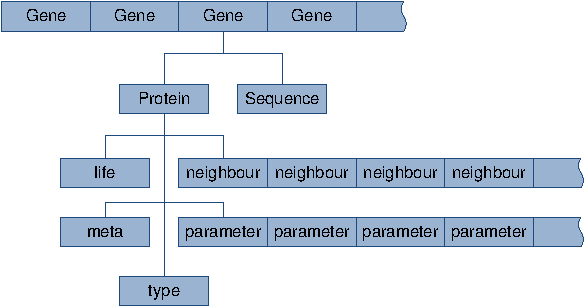
\includegraphics[scale=1.2]{artdev3d_genotype}
	\caption{Genotype representation in ArtDev3D}
	\label{fig:artdev3d_genotype}
\end{figure}

The genotype of this model (see fig~\ref{fig:artdev3d_genotype}), the DNA, is an array with genes. The genes carry a recipe for a protein and a genetic sequence. The gene sequence is used to find genes with desired proteins to synthesize. The protein type determines what its function is. If a protein that changes the cell's type is a type, then proteins that regulate chemicals are another. How the protein is activated, is stored in the neighbours and chemicals array. The neighbours array stores the desired types of nearby cells. The neighbourhood in this model is defined to be the cells that a cell are in direct contact with in free space. That is above, below, left, right, front and back. The chemicals array stores the desired chemical levels in the cell. Once nearby cells' types correspond to the neighbourhood criteria, and the chemical levels in the cell are equal to or above the criteria of the protein, it is activated. Data in \texttt{meta} contains only one of two things, a cell type or a genetic sequence. These are used by the cell-type-changing and transcribing proteins respectively. The regulating and growth proteins only use the parameters. Figure~\ref{fig:artdev3d_protein-parameters} shows how the parameters are used to store the values to adjust the chemicals in a cell. Likewise, the proteins can store stimuli for each direction it wishes the cell to duplicate to.

\begin{figure}[!ht]
	\centering
	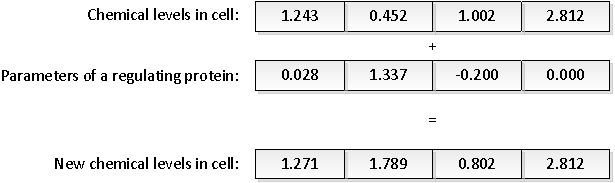
\includegraphics[scale=1.2]{artdev3d_protein-parameters}
	\caption{Parameters representation in ArtDev3D}
	\label{fig:artdev3d_protein-parameters}
\end{figure}

The genes are implemented this way in order to make it possible to copy whole genes during cross over, while at the same time, opening up the possibility to mutate any of these properties.

\subsubsection{Development}
Development starts with an ``empty'' organism. The genotype, or the DNA, is copied into a cell, which is then inserted into the organism. The organism now contains a single cell with DNA. Since this is the first cell, there is a special routine that will take place. The cell will ``scan'' through the DNA and synthesize all proteins it can find. This is the initialization stage. Once completed it is ready for development. Every development step, all cells will execute the same set of operations as follows:

\begin{enumerate}
	\itemsep=0pt
	\item Determine which proteins are active.
	\item Have all active proteins request an action.
	\item Accumulate actions and execute them.
\end{enumerate}

Note that while the DNA indirectly requests actions upon the cell through the proteins, the cell performs the real work like regulating the chemicals and proteins behind the scene. The cell functions limit what the DNA can do, but at the same time, the DNA can affect both the cell and its surroundings using proteins as its proxy.

The development ends when a number of steps have passed, and the organism is rated based on how similar it is to the target phenotype. In this case, the targets are usually simple three-dimensional shapes.

While working with this model, it was discovered that the development algorithm does not develop all cells simultaneously. Usually, all cells must receive or gather information on nearby cells before any actions are executed. This is not the case here. Every cell gathers information and executes action in one go. So when the next cell gathers information, there will be ``new'' information mixed in. This flow is described in more detail in chapter~\ref{sec:Implementation:ArtDev3D}. However, the model seem to work rather well regardless. Besides being able to develop target shapes, H{\o}ye's experiments also showed a number of interesting things. The initial number of don't-care-neighbours, i.e.\ the number of neighbours that can be of any type, had a negative impact on the growth of an organism when lowered. It was clearly best to make the first few cells indifferent to the neighbouring cells' types. It was also shown that having a higher number of chemical types in the cells only contributed to making it harder to correctly develop the target shapes. This is most interesting because this is a clear contradiction to the results achieved by the model we are going to discuss in the following section. It is inspired by intercellular communication by means of chemicals and types of nearby cells, and has been shown to work very well.


\subsection{Artificial Development (ADCGP)}
Artificial development using Cartesian genetic programming is built on a genetic program invented by Julian Miller in 1998. The following description of what the model is and how it works is based on a number of articles, but mostly from \cite{mteurogp2000} and \cite{ecal2003}. There may therefore be discrepancies compared to his latest work. The model is based on developing a feed-forward graph that maps an input to an output, or a digital circuit in a layman's term.

\subsubsection{Concepts}
The model focuses a great deal on intercellular communication. In biology, this is achieved by means of secreting chemicals through the cell's membrane. The same membrane is also used to receive chemicals from other cells. Based on the presence of some chemicals and the types of nearby cells, a cell will perform a set of operations to see if a change in cell type is needed, and in which directions it should divide itself to.

\begin{figure}[!ht]
	\centering
	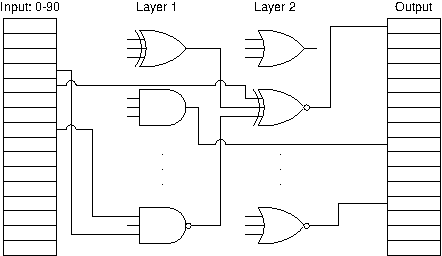
\includegraphics[scale=1.7]{cartesian_genotype}
	\caption{Genotype representation in artificial development}
	\label{fig:cartesian_genotype}
\end{figure}

The genotype of this model (fig.~\ref{fig:cartesian_genotype}) is a string of numbers that make up a feed forward circuit. This is represented as a set of four numbers where the first three point to a node, and the last number denotes which function to perform. The input to this function is the output of the nodes that the first three point to. We will see what this means in a moment.

In the simplified figure above (some gates aren't connected to avoid clutter), the input string consists of 90 bits, denoted 0 up to and including 89. Every gate, or node, are denoted 90-\emph{n}, where \emph{n} is the number of nodes. This means that the first gate we see in layer 1, is denoted 90, and the one under it is 91. Now we look at the genotype. As mentioned, it consists of four numbers. 7, 50, and 32 point to the corresponding bits in the input string, i.e.\ 7th, 50th and 32nd bits of the input string on the left. These bits are fed to the gate with a function identified by the fourth number. In this case, it is 10, or an XOR gate. If an input number was higher than 89, it would be pointing to the output of a gate instead of the input string. The second node in layer two, gets its inputs from two nodes in the first layer. The last few numbers of a genotype do not describe a circuit. They still point to different bits, but they are no longer inputs to a function. These bits will make up the output string instead. Note that the number of inputs to any gate, can be of any number as long as it is greater than 2, and is consistent.

As opposed to ArtDev3D, every cellular activity is evolved. Nothing is programmed directly into the cell. Consequently, the evolved cell program can be difficult to analyze. The gates seen in the figure, if written down, are just a series of Boolean operations with no apparent meaning to the average human mind.

\subsubsection{Development}
There are several ways to start development with this model. One way is to represent the organism as a 2d grid filled with cells and alternately give them maximum and no chemicals. If the grid was a chess board, the white cells will have maximum chemicals and the black ones have none. The other way, and the way it is implemented here, is to start like ArtDev3D with a single cell in the centre and give it a maximum amount of chemicals. The cell program can then be executed. As the cell program is implemented entirely by evolution (and chance), explanation of what happens inside the cell is nearly impossible. Whatever happens in the cell, the output will determine whether or not the type of the cell should change, whether the cell should perform division in a direction, and how much chemicals the potentially new cell should be given.


\subsection{A generic development framework}
\label{sec:framework_requirements}
Clearly, there are many differences that can make it difficult to compare these two models. As can be seen above, there are many biological concepts used in the models that do not overlap. They are based entirely on different ideas, and on top of that, are implemented differently. In one model the cell program is evolved through many generations to achieve intended effect, while in the other, the cell does not have a program in the same sense. It is present only to do the DNA's bidding. The program is not subject to change, only the DNA is. The most prominent difference between the two, however, is perhaps how cellular interaction takes place, and the results they've been given.

In ADCGP, the cells communicate with each other using chemicals. The amount of chemicals exchanged, along with nearby cells' types determine what will occur in the cell in a development step. In ArtDev3D, communication happens without the chemicals. The state of the neighbourhood alone make up the external signals that contribute to determine whether or not some proteins are activated. Chemicals in ArtDev3D are used internally only and are not exchanged. Furthermore, it has shown that the number of chemical types is inversely related to fitness. Quite the opposite of how ADCGP is reported to work. One can place these models in their own end of the scale. Because of this controversy, there are discussions as to whether chemicals really are necessary.

These are only two models in a relatively new field where a lot of research is still ongoing. How can we tell why something is working for one model, and not for the other? What will happen when a third model gives a third result? These kinds of questions can be difficult to answer to any degree of certainty with so many factors to consider. But these are the kinds of questions that one may want answers for.

To solve this problem, one can try and nullify the impact these factors. In order to do so, there is a need to identify which factors are in fact having this kind of an effect on a model. Once identified, these factors can be nullified by making it equal for all models. This means, for instance, that a definition or concept used in artificial development, must be the very same in all models. As long as the definitions and/or concepts are generic enough, this should pose no problem for any model. This thesis proposes a framework that will provide such a structure, and that is generic enough for any development model, all without forcing any comprimises. Any model implemented within this framework will have a much clearer structure, making it much easier to make comparisons and studies. The following points are requirements for what such a model should include, and why they are identified as a difference factor:

\begin{itemize}
	\item\textbf{An evolutionary algorithm}

	Using a common algorithm will eliminate discussions on whether or not a certain algorithm is better than another. The focus should be on the development model, and not the genetic algorithm that doesn't work very well for one model.

	\item\textbf{A development algorithm}

	Most of the models use the same basic algorithm for development, i.e.\ with every development step, every cell in an organism is told to execute their program. This occurs for a configurable number of steps, and varies very little from model to model. Hence, there is no need to implement this algorithm every time, making models different for no good reason. In cases such as with ArtDev3D, this will automatically address the issue with simultaneous cell development as well.

	\item\textbf{A common messaging system}

	Especially with these two models, there are different things that go into a message that is sent to nearby cells. A common message should be able to contain most of a cell's properties while constrict the messages to just that and nothing more. The user can just choose the relevant parts of a message for his or her model. When comparing, one should be able to say that two models differ because one uses chemicals while the other uses both chemicals and cell types. This is made possible because they are both still using the same message, only not all parts of it.

	\item\textbf{Common implementation of concepts}

	It is important that a cell is always a cell, regardless of which model we are talking about. The definition of a cell should not change because a model wants it differently. Likewise, there should be only one definition for chemicals, organisms and proteins. While they are restricted and enforced on the user, it should also be generic enough to implement any model.

	\item\textbf{Protecting the organism}

	Access to the organism should be limited to avoid accidental tampering. Cell division should occur by telling the organism, through a function call, to add a cell in a particular location. All information regarding the cellular neighbourhood should already be available through the messaging system. As such, mechanisms should also be available to check whether a cell in a particular location exists or if it will be occupied by a new cell. This is to enable checks prior to performing cell division.
\end{itemize}

There are several benefits to using such a framework. First and foremost, it will cut down on implementation time. Such a model will allow a user to concentrate wholly on their model and not spend time implementing the most suitable evolutionary algorithm, or finding out whether or not the messaging system was implemented correctly. Instead, the user need only use what is already there and just fill in the blanks. Secondly, the implementation can be guaranteed to work. As the framework matures, the user can be assured that if something does not work, it is most likely their model and not because of a bug elsewhere in the system. This is a typical scenario with independent implementations. Finally, and probably most importantly, the framework will hopefully be able to reduce the number of factors that have an effect on the outcome of a model. This reduction will consequently lead to clearer studies and better results.

We've seen that these two models are quite different from one another, which is why they will serve as an excellent starting point to implement the framework. As one of the criteria for the framework is to be generic, this will form the first step towards that important requirement. However, being able to implement these models does not mean everything. It should also be able to perform just as well as these did originally. There is no point in having a fancy framework like this, if it cannot deliver as well. We will take a look at this later. First, we will have a look at the implementation of the framework, and re-implement these two models within the framework.
